\chapter{Implemented Modules} \label{ch_4:chapter}

In this chapter, the technical goals of the project are introduced. Each developed module will be explained as well as it's requirements and specification details. For each module, the following points will be addressed:

\begin{itemize}
  \item Technical goals
  \item Problem to which the module provides a solution
  \item Some of it's properties (reusability, scalability \dots)
  \item Integration with the current version of Aerostack
\end{itemize}

The chapter is structured as follows: Section \ref{ch_4:sect:requirements} presents the requirements imposed for the implemented modules, explaining the specifications for Aerostack modules \ref{ch_4:subsect:specs} and its integration \ref{ch_4:subsect:integration}. Sections \ref{ch_4:sect:behav_slam} and \ref{ch_4:sect:nav_interface} explain the slam behavior and the navigation API respectively and \cref{ch_4:subsect:behav_gtp,ch_4:subsect:behav_fpog,ch_4:subsect:behav_gpog,ch_4:subsect:path_planner} go through the rest of behaviors, explaining its particularities.

\section{Requirements} \label{ch_4:sect:requirements}

  In order for the Aerostack framework to localize with a different technique rather than visual markers, a lidar sensor will be used. In this case, the \textit{Hokuyo Eye} range sensor will be employed, which is the \textit{defacto} range sensor in this context. Also, the low level implentation provides a nice ros API that can be used to fetch data. To wrap all this functionallity we propose the implementation of a new high level behavior that coordinates all the framework with the lidar interface, providing a high level, standarized API for lidar-based localization.

  As of the current version of Aerostack, navigation is done with a 2D probabilistic roadmap planner, the input for the planner is a predefined map, done by hand in the Graphical User Interface that Aerostack provides. This is a static map and goes against the nature of the any dynamically acquired mapping signal. To tackle this problem several new navigation behaviors are proposed. These behaviors will abstract the planner used for each localization mode, providing a high level standarized API that can be used independently of the localization technique, replacing the old one.

  \subsection{Specification} \label{ch_4:subsect:specs}

    Each implemented module should follow the specification imposed by the Aerostack framework. In Aerostack there are different types of processes providing structure and added functionallity. When a new process is created it should be decided whether to implement it as a plain, simple ros node, a robot process or a behavior process. Their differences are as follows:

    \begin{itemize}
      \item ROS Node: This is the standard way of adding modules in a ROS oriented architecture. A ros node is simply a process programmed in any of the programming languages supported by ros (C, C++, Python \dots) that implements a task and is interfaced through the ros master server with named topics, services or both. A ros node can subscribe or publish topics and optionally, provide services, as many topics or services as it wants. These topics and services are nothing more than binded ports to the ROS master server, that works over TCP (normally) or UDP to distribute traffic. This is the implementation to follow when adding very low level modules, like platform drivers.
      \item Robot Process: A Robot Process is an abstraction provided by Aerostack, it serves mainly as a standarization layer, providing an interface for the rest of the architecture to be used. It provides three services to manage the process, one for stopping it, one for starting it and another one to check whether it is running or not, aditionally it emits an alive signal every second or an error signal when the thread crashes. It runs the inheritors' code inside a separate thread in order to monitor it. When adding a module that abstracts some low level APIs, like a visual marker processor, this is the class to inherit from.
      \item Behavior Process: This is the highest level of the hierarchy, inside the Aerostack framework there exists a process that coordinates all the behaviors, to do so, every behavior exposes an interface similar to the Robot Process and a configuration file that especifies the mid and low level processes the behavior depends upon (it's capabilities and incompabilities), amongst other parameters, in this sense, the behavior that provides localization based on visual markers depends on the visual marker processor to work. Formally, a behavior is just a high level process that monitors an algorithm: it runs the algorithm in a separate thread and emits the state and error signals, listening to \textit{start/stop} events and acting accordingly over the algorithm. When adding a high level functionallity, this is the class that should be inherited.
    \end{itemize}

    In a similar fashion to the visual marker localization behavior, the lidar localization behavior proposed will require three more processes: the slam process, an ekf that combines various signals and a localization technique selector, this is explained in detail in the corresponding behavior section (sect. \ref{ch_4:sect:behav_slam}).

    The navigation interface is slightly more complicated, it will be composed of various behaviors that provide different functionallity, abstracting away the logic needed to navigate at different levels. We propose three new behaviors and the inclusion of a new planner, efficiently designed to work with lidar signal. More details will be provided in the corresponding section \ref{ch_4:sect:nav_interface}

  \subsection{Integration} \label{ch_4:subsect:integration}

    To integrate each behavior, we will follow a bottom up procedure. This way, we will ensure that the processes the behavior depends on are working correctly inside the Aerostack and the error doesn't get masked with the behavior integration.

    When integrating a new behavior some steps should be followed:
    \begin{itemize}
      \item Add the necessary mid and low level processes to the Aerostack and ensure they can be started automatically.
      \item Add the technical specification of the behavior to the behavior catalog. These are the capabilities and incompabilities of the behavior and should include the mid and low level processes previously mentioned so that they can be started automatically. In this step, the behaviors that are incompatible with the new one should be identified.
      \item Add the implementation of the behavior and test it with the Aerostack to ensure it can be started and that no incompatibilities arise.
    \end{itemize}

    The lidar-based localization behavior will provide a new localization mode, so it is reasonable to mark the rest localization behaviors as incompatible, also, a new localization method selector process will be added, this will ensure that when various localization techniques are to be used in the same mission, they can be easily toggled on and off. This will be detailed in the corresponding behavior section \ref{ch_4:sect:behav_slam}.

  \pagebreak

  We can define the requirements for these modules more formally, in a global sense, the new functionality added should meet the following requirements.
  
  \begin{enumerate}
    \item It should be able to handle lidar sensor input and use it both to localize and map.
    \item It should be able to do planning with the available data to get to a desired goal avoiding obstacles.
    \item It should be able to adapt in environments with moving obstacles.
    \item It should be efficient enough to run both onboard and on ground control stations.
    \item It should be possuble to be interfaced at different levels of abstraction.
    \item It should provide an standarized API access to navigate the robot using lidar sensorization.
  \end{enumerate}

\section{Behavior Self Localize and Map by Lidar} \label{ch_4:sect:behav_slam}

  The lidar range sensor outputs raytraces reflected over the near objects, in a way, it resembles a sonar sensor (that's way it's called lidar). Each raytrace, measures the distance from a concrete angle to a point at a certain distance, these measures then have to be converted in some way that can be used to map the environment and use this mapped environment to localize inside it (see section \ref{ch_3:sect:localization:slam} for an in-depth explanation of SLAM). Refer to figure \ref{ch_4:fig:behav_slam} for a visual representation of the behavior and it's subprocesses.

  We will use a ros module developed at the Darmstadt University that provides a SLAM node (\textit{hector\_mapping} \cite{hector_slam}). Taking the lidar's cloud of points it is able to construct an occupancy grid map and then localize inside it (SLAM). The output of this module can be used to create a plan avoiding obstacles to reach a target point. It will output the estimated localization along with the mapped environment. This localization will be merged with the measures from the rest of the sensors (namely odometry, IMU \dots) using an extended kalman filter (see section \ref{ch_3:sect:localization:ekf}) to output a robust estimate of the robot's position inside the mapped world. 

  The process in charge of the EKF is called \textit{droneRobotLocalization} and inherits from \textit{Robot Process} class. It will listen for updates on the robot's pose (\textit{hector\_pose} topic) and both the IMU and the odometry topics and output the estimated pose.

  \begin{figure}[h] 
    \centering
    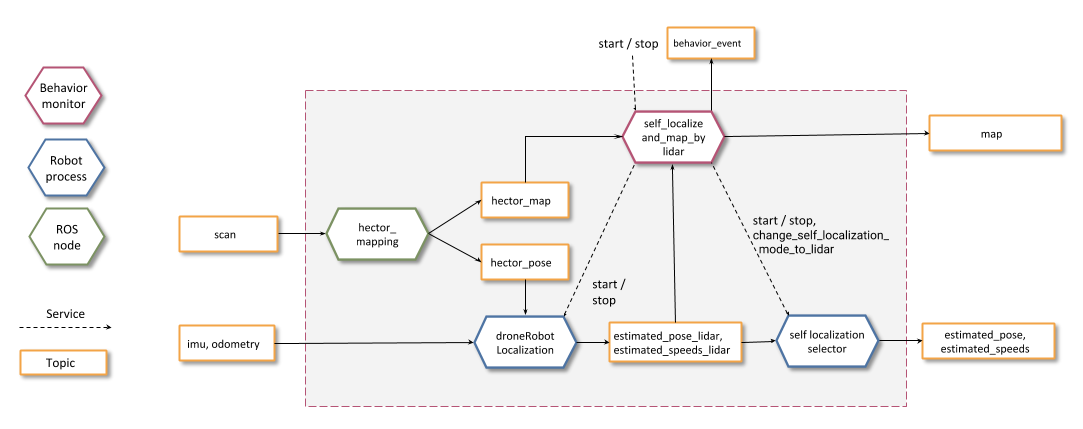
\includegraphics[width=\textwidth]{./Figures/BehaviorSlamArquitecture.png}
    \caption{Behavior self localize and map by lidar architecture. \textit{Hector mapping} is the SLAM module from \cite{hector_slam}. \textit{Drone Robot Localization} does the EKF. \textit{Self Localization Selector} gives the localization based on the selected technique.}
    \label{ch_4:fig:behav_slam}
  \end{figure}

  The estimated pose is then fed to the selector, which will toggle the localization technique. This implementation opens the door to new localization behaviors, a GPS based one for instance and also makes compatible the previous ones (visual markers or odometry based). It is easy to think of an scenario that requires both indoor and outdoor localization, in such a mission, the localization technique in use should be toggled in order for the navigator to work properly. As can be seen in Fig. \ref{ch_4:fig:behav_slam}, this is a \textit{Robot Process} with an added service to change the localization technique used.

  Bellow there is a list of the inputs and outputs of this behavior:

  \begin{itemize}
  \item scan: This is the output of the lidar node, it is directly fed into the \textit{hector mapping} node
  \item imu: This topic contains the measures from the \textit{inertial measurement unit}
  \item odometry: This is a general topic with the measures from odometry
  \item map: This is the map as processed by the \textit{hector mapping} node
  \item estimated\_speed\_lidar: This is the estimated speed from the whole behavior process, fed to the selector
  \item estimated\_pose\_lidar: This is the estimated pose from the whole behavior process, fed to the selector
\end{itemize}

  This behavior monitors the correct working of the algorithm (\textit{hector mapping}) by listening on the \textit{map} topic, when it outputs strange or simply wrong data, an error is emitted.

  In the configuration file of this behavior the localization by visual markers behavior will appear as incompatible. As for the capabilities, all of \textit{hector mapping}, \textit{drone robot localization} and \textit{self localization selector} will figurate as capabilities, indicating that those processes should be started before this behavior. Furthermore, when it's activation conditions are tested (\textit{checkOwnActivationConditions}, native method each behavior should implement), it will check that the robot actually counts with a lidar interface. All these configuration parameters are depicted in figure \ref{ch_4:fig:behav_slam_catalog}.

  \begin{figure}
    \centering
    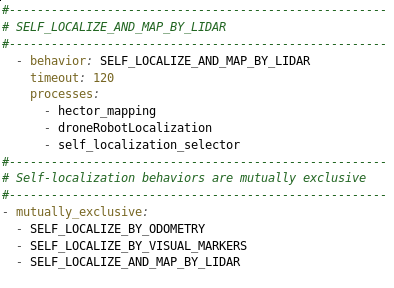
\includegraphics[height=0.25\textheight]{./Figures/BehaviorSlamCatalog.png}
    \caption{Self Localize and Map behavior catalog specification. Required processes and timeout values are specified.}
    \label{ch_4:fig:behav_slam_catalog}
  \end{figure}

  The monitor algorithm will consist in checking the consistency of the output map as well as it's frequency, when a drift is detected a warning will be printed, indicating that the slam module is having problems. In the worst case, when the node does not output a map at all, an error will be emitted and the behavior will terminate.

\section{Navigation Interface} \label{ch_4:sect:nav_interface}

  We will consider the navigation interface as the minimum set of behaviors necessary to provide a robust, flexible API to do navigation tasks related to lidar-based localization and mapping techniques. It should be able to generate obstacle-free trajectories  to any given point (when there exists one) and be able to move the robot along those trajectories.

  The identified tasks for this API are as follows:

  \begin{enumerate}
    \item Given a point (or goal), execute the necessary motions to get the robot to that goal.
    \item Given a path, execute the necessary motions to follow it until the path is finished.
    \item Given a point (or goal), generate an obstacle-free path from the current robot's position to that goal.
  \end{enumerate}

  This tasks can be directly mapped with processes. However, we will implement them as separate behaviors to provide more modularity and reusability. Also, as each process will provide abstraction at a certain level of granularity, it makes sense to implement it as separate, independent behaviors (although some code will be duplicated)

  As of the current version of Aerostack, there exists a behavior that executes the motion of going to a given point in the 2D map representation used by Aerostack. However, this behavior is not general enough to be used with a different map representation, so we will implement a new one capable of executing the motion in the new map format: occupancy grids (which is the format used in \textit{hector mapping}). Also, in a dynamic environment, obstacles can arise in the path, this behavior will ensure that no collisions happen when executing the motion. More details to follow in section \ref{ch_4:subsect:behav_gtp}.

  The task of following a path or trajectory consists in instructing the previously available trajectory controller to follow a set of points (that conform the trajectory), given in a specific reference frame (world coordinates in this case). Contrary to the previously defined behavior, this one executes the motion blindly, providing a lower level of control to the user. Please refer to \ref{ch_4:subsect:behav_fpog} for more details.

  For the last functionality, generating obstacle-free paths, another behavior will be implemented. It will consist mainly in a wrapper around the new planner, providing the lowest level of control in our navigation interface. For the planning we will employ the previously mentioned planner \textit{move base}, provided as a ros package, which is specially crafted for lidar interfaces. It accepts an occupancy grid map and the raytraces from the lidar and implements the planning algorithm. Under the hood, it uses the elastic band algorithm for path optimization, as mentioned in section \ref{ch_3:sect:planning}.

  The proposed names for each behavior are: \textit{behavior go to point in occupancy grid}, \textit{behavior follow path in occupancy grid} and \textit{behavior generate path in occupancy grid}. \cref{ch_4:fig:behav_gtp,ch_4:fig:behav_fp,ch_4:fig:behav_gp} ilustrate the architecture followed by each of these behaviors. The following subsubsections explain each behavior in detail.

\subsection{Behavior Go to Point in Occupancy Grid} \label{ch_4:subsect:behav_gtp}

  This behavior provides the highest abstraction level of all the navigation interface, provided a target point, it will generate an obstacle-free trajectory to follow and send it to the trajectory controller, which executes the necessary motions to follow that trajectory. During the motion, this behavior will also ensure that no dynamic object gets in the way, recalculating the trajectory if necessary. In order to plan the trajectories, the new planner, \textit{move base} will be used, and as it will be a goal based behavior, the taget goal will be given as an argument to the start service. Figure \ref{ch_4:fig:behav_gtp} illustrates the general architecture of this behavior.

  \begin{figure}[h]
    \centering
    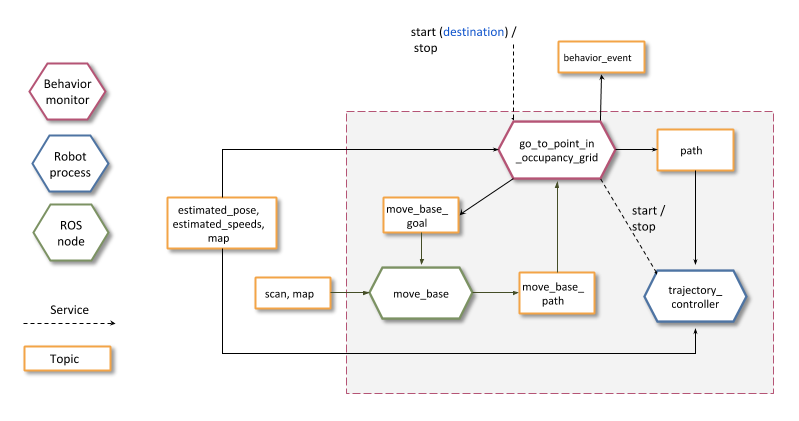
\includegraphics[width=\textwidth]{./Figures/BehaviorGTPArquitecture.png}
    \caption{Behavior Go to Point architecture. Move base is the planner}
    \label{ch_4:fig:behav_gtp}
  \end{figure}

  A condition for this behavior to operate correctly is that no other behavior is instructing the trajectory controller. To ensure this condition is met, the list of motion behaviors is stated as incompatible. The capabilities should list that it is a set-point-based flight behavior, instructing the behavior coordinator to setup the trajectory controller accordingly, the new planner (move base) should be explicitly declared as well so it is started automatically. Figure \ref{ch_4:fig:behav_gtp_catalog} depicts the part of the global configuration file pertaining this behavior. Using four parameters as input enables the behavior to accept orientation (yaw) commands as part of the goal, making the behavior more flexible.

  The proposed topics will be:

    \begin{itemize}
    \item \textbf{scan}: Scan data from the lidar, direct input to the planner.
    \item \textbf{map}: Occupancy grid map from the self localize and map by lidar behavior, direct input to the planner.
    \item \textbf{pose, speed}: Estimates of the current robot's position and speed.
    \item \textbf{move base goal}: Topic to instruct the planner to calculate an obstacle-free trajectory. Used by the path planner module.
    \item \textbf{move base path}: Topic with the planned trajectory from the move base module. Grabbed from the path planner module.
    \item \textbf{candidate path}: Output topic with the candidate trajectory, output from the path planner, grabbed from the behavior to instruct the trajectory controller.
  \end{itemize}


  \begin{figure}[!h]
    \centering
    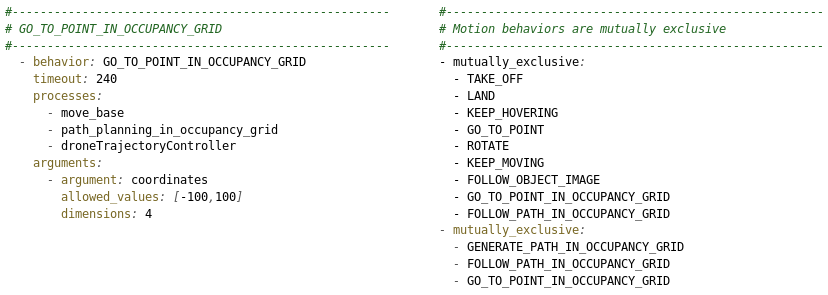
\includegraphics[width=\textwidth]{./Figures/BehaviorGTPCatalog.png}
    \caption{Go to Point behavior catalog specification. Required processes and timeout values are specified.}
    \label{ch_4:fig:behav_gtp_catalog}
  \end{figure}


  The process \textit{path planning in occupancy grid} is in charge of monitoring the \textit{move base} planner, it's the intermediary between any behavior requesting a trajectory plan and the planner itself. It is explained in detail in section \ref{ch_4:subsect:path_planner}.

  When the behavior is started it receives an absolute or relative coordinate to go, it waits for the current position estimate and starts planning. If the robot's orientation has to be changed it first instructs the trajectory controller to do so, until the target orientation is achieved. Once the robot is correctly oriented, the path planner is asked for a candidate path to follow and the trajectory controller is instructed to follow it. Also, while the trajectory is being executed, the behavior still listens to new paths, this way, when the planner outputs an empty trajectory we know that an obstacle is obstructing the path, stop the controller and replan again. 

  This strategy for detecting obstacles comes from the fact that the newly integrated planner outputs an empty path when an obstacle is found on the way.

  As for the activation conditions, this behavior requires that the battery is not in a \textit{LOW} state and the aircraft is in state \textit{FLYING}. To check these conditions, it will make use of the \textit{belief manager} that stores important state information from all the Aerostack in the so called \textit{beliefs}. Beliefs are the symbolic representation of the known environment and gathered information so far in the mission, they are the other part of the executive layer, providing persistance accross the whole mission. For example, when the drone starts flying it will toggle its state from \textit{LANDED} to \textit{FLYING} and the belief manager will gather this information for easy retrieval, this goes for the battery state too.

\subsection{Behavior Follow Path in Occupancy Grid} \label{ch_4:subsect:behav_fpog}

  This behavior will communicate with the trajectory controller, instructing it to move following a given path received as an input argument. For this behavior to work correctly, the motion behaviors should be disabled too. In this case, no other low level process is needed. The following figure illustrates the general concept (\ref{ch_4:fig:behav_fp}). Following a path can be a useful feature when developing fine grain controlled missions, like the ones enabled with Python.

  \begin{figure}[h]
    \centering
    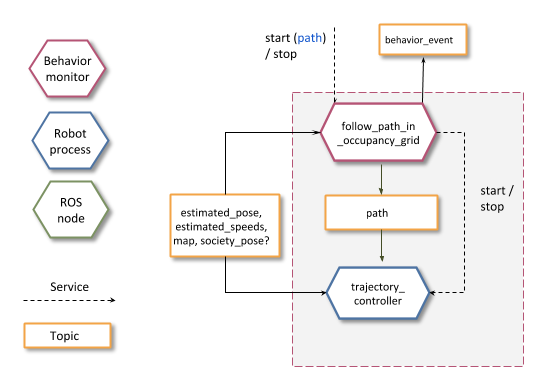
\includegraphics[width=\textwidth]{./Figures/BehaviorFPArquitecture.png}
    \caption{Behavior follow path in occupancy grid architecture}
    \label{ch_4:fig:behav_fp}
  \end{figure}

  The important topics are explained below:

  \begin{itemize}
  \item \textbf{pose, speed, map}: These are the input topics both for the trajectory controller and the behavior.
\end{itemize}


  Again, the correct settings should be ensured in the configuration file, marking motion behaviors to avoid trajectories interferences. This settings can be observed in figure \ref{ch_4:fig:behav_fp_catalog}.

  \begin{figure}
    \centering
    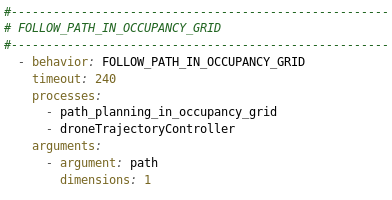
\includegraphics[width=\textwidth]{./Figures/BehaviorFPCatalog.png}
    \caption{Follow Path in Occupancy Grid behavior catalog specification. Required processes and timeout values are specified.}
    \label{ch_4:fig:behav_fp_catalog}
  \end{figure}

  This behavior has similar constraints to the previous one, if the aircraft battery is low or is landed, it cannot be executed. In this case, the monitor is much simpler, given a trajectory it instructs the trajectory controller to follow it, not even listening to path events. Not avoiding obstacles was a design decision taken to promote developers independence and granularity control. When the behavior starts, the provided path will be parsed into a known data structure, if no path is given or it is malformed an error will be thrown and the behavior will finish.

\subsection{Behavior Generate Path in Occupancy Grid} \label{ch_4:subsect:behav_gpog}

  In this case we will only implement a wrapper around the path planner module. This is the lowest abstraction level behavior provided by the navigation interface API. Being able to generate paths can be useful for fine grain controlled missions and debugging. The only communication way for this behavior will be dropping the planned path on the belief memory, this way the amount of traffic and topics is reduced, saving computing resources and avoiding polluting more topics. It's architecture is depicted in figure \ref{ch_4:fig:behav_gp}.

  \begin{figure}[h]
    \centering 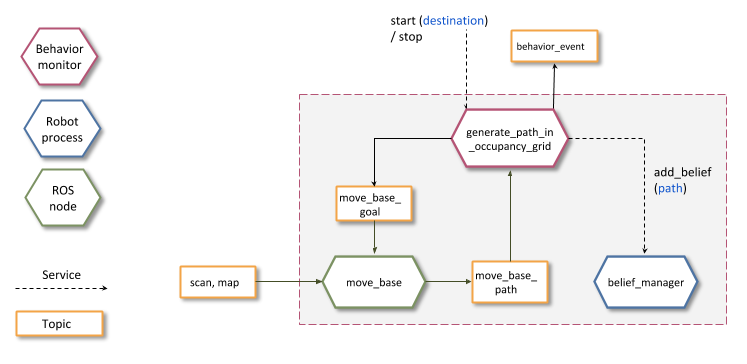
\includegraphics[width=\textwidth]{./Figures/BehaviorGPArquitecture.png}
    \caption{Behavior generate path in occupancy grid architecture}
    \label{ch_4:fig:behav_gp}
  \end{figure}

  Contrary to the rest of the presented behaviors, as this one does perform any motion, it does not have any restriction, nor it conflicts with any behavior requiring the trajectory controller. This behavior will store any given path in the belief memory with a different unique identifier, ensuring that the computed paths are not smashed, this is a desirable feature for many reasons, the most obvious being able to avoid the overhead of planning again, reusing precalculated paths. This allows for a developer to execute a trajectory by parts for example. Figure \ref{ch_4:fig:behav_gp_catalog} overviews the part of the catalog dedicated to this behavior.

  \begin{figure}
    \centering
    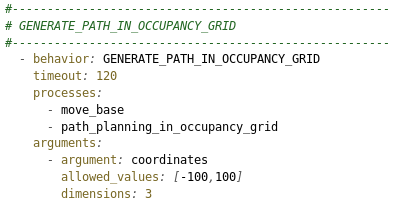
\includegraphics[height=0.19\textheight]{./Figures/BehaviorGPCatalog.png}
    \caption{Generate Path behavior catalog specification. Required processes and timeout values are specified.}
    \label{ch_4:fig:behav_gp_catalog}
  \end{figure}

\subsection{Path Planner in Occupancy Grid} \label{ch_4:subsect:path_planner}

  This module was developed as part of the Navigation Interface to provide a unified API access to the move base planner, reducing the overhead of changing the planner in the future and monitoring the correct funcioning of the move base planner.

  It implements a queue of target goals and dispatches them one by one to the planner. This decision was taken for two reasons, the main one is that \textit{move base} contains a bug, when the computation power is lowering, sometimes the planner fails to generate a path. To monitor this strange behavior and correctly handle it we implemented this intermediate module. The second reason is that in the future, the underlying planner could be changed, unifying a path planning API will smooth the transition, making it transparent to the API consumers.

This chapter has reviewed the most important aspects and specification of the implemented modules. In the next one, the validation and testing for these behaviors will be introduced.

